\section{Periodogram-based Methods Applied to Real–World Data}

\begin{enumerate}[label=\alph*), leftmargin=*]
%% a)
\item
%

The sunspot time series and its Chebyshev-windowed periodogram method are provided at figure \ref{fig:1_4_a}.
The raw time series (blue) spectral estimates are compared to two preprocessed series:
\begin{enumerate}
    \item a centered and detrended series (red, \texttt{mean \& detrend})
    \item a logarithmic centered series (yellow, \texttt{log \& mean})
\end{enumerate}

\begin{figure}[h]
    \centering
    \begin{subfigure}{0.49\textwidth}
        \centering
        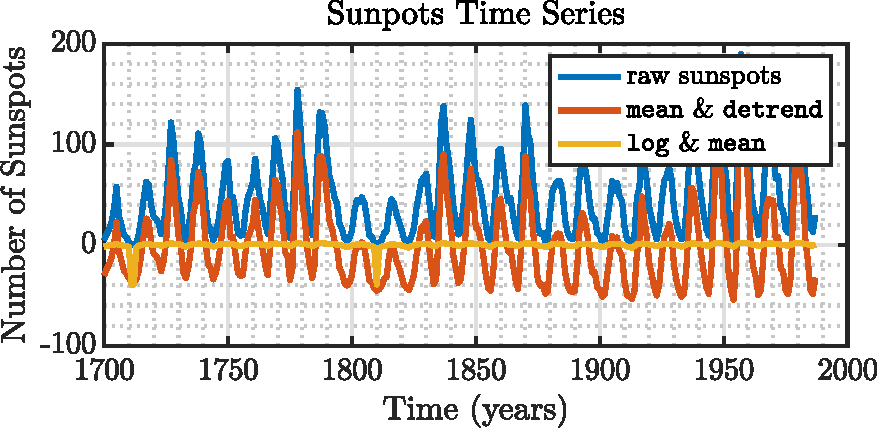
\includegraphics[height=1.5in]{report/spectrum-estimation/periodogram-based-methods-applied-to-real-world-data/assets/a/sunspots-raw}
    \end{subfigure}
    ~ 
    \begin{subfigure}{0.49\textwidth}
        \centering
        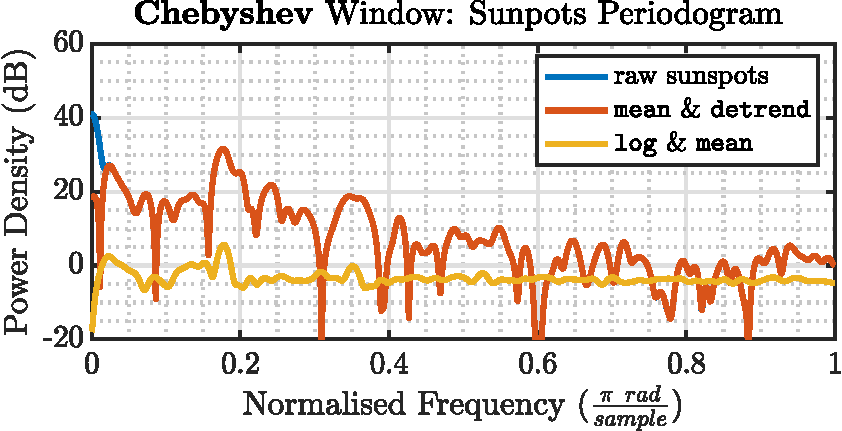
\includegraphics[height=1.5in]{report/spectrum-estimation/periodogram-based-methods-applied-to-real-world-data/assets/a/sunspots-Chebyshev}
    \end{subfigure}
    \caption{Sunspots: Chebyshev-windowed periodogram method, to raw and preprocessed series.}
    \label{fig:1_4_a}
\end{figure}

Subtraction of the \texttt{mean}, results in attenuation of the DC component ($f = 0$), while \texttt{detrend} removed low-frequency components.
Consequently, the spectral estimate of the centered and detrended series is almost identical to the raw sunspots time series for frequencies $f \gtrapprox 0.02$ (in $rad/sample$),
while the lower frequency components are eliminated.

To avoid logarithms of zero, the logarithmic series is obtained by first adding a small constant to the raw sunspots time series (MATLAB $\mathtt{eps} = 2.2204e-16$) and then
taking natural \texttt{log} and removing the \texttt{mean}. Similarly, the DC component is also removed and the peaks at the same frequencies are observed, but now they are more noticeable
(only peaks of interest are above $0dB$).

%% b)
\item
%

The Standard and Bartlett method periodograms of the EEG signal are provided at figure \ref{fig:1_4_b_1}. The latter is easier to interpret since its peaks are accentuated.
The peaks distinguished from the periodograms are at frequencies $f = 13,\ 26,\ 39,\ 50\ Hz$ as well as a wider peak at $8-10\ Hz$.

\begin{figure}[h]
    \centering
    \begin{subfigure}{0.49\textwidth}
        \centering
        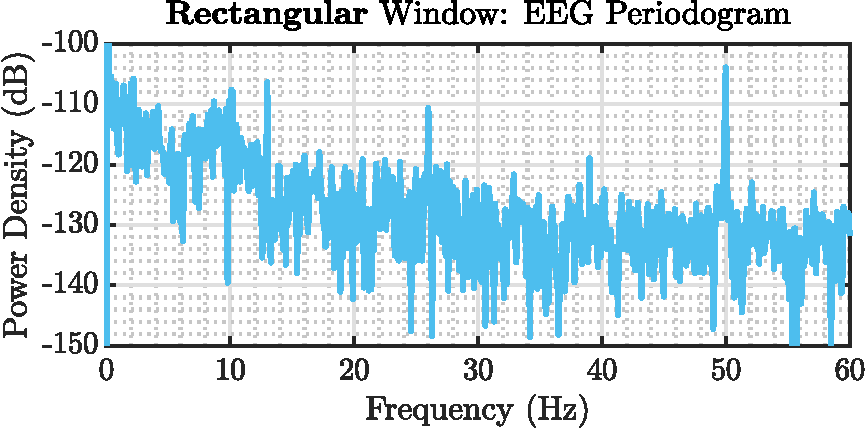
\includegraphics[height=1.5in]{report/spectrum-estimation/periodogram-based-methods-applied-to-real-world-data/assets/b/eeg-periodogram-standard}
    \end{subfigure}
    ~ 
    \begin{subfigure}{0.49\textwidth}
        \centering
        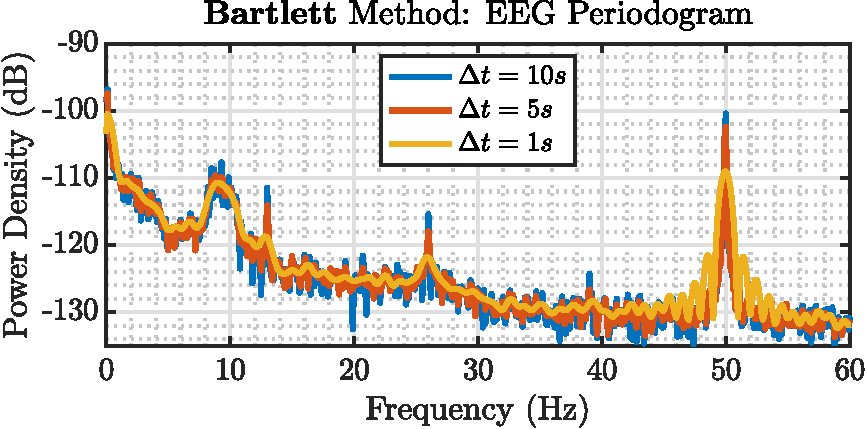
\includegraphics[height=1.5in]{report/spectrum-estimation/periodogram-based-methods-applied-to-real-world-data/assets/b/eeg-periodogram-averaged-bartlett}
    \end{subfigure}
    \caption{EEG: standard and Bartlett method periodogram.}
    \label{fig:1_4_b_1}
\end{figure}

As suggested by the instructions, the components in $8-10\ Hz$ are due to the tiredness of the subject during the recording, adequately captured by the Bartlett method periodograms,
regardless the window length $\Delta t$.

The peak at $f_{0}^{SSEVP} = 13\ Hz$ corresponds to the fundamental frequency of the SSEVP, whose harmonics can be noticed at frequencies $f_{1}^{SSEVP} = 26\ Hz$ and
$f_{2}^{SSEVP} = 39\ Hz$. Its third harmonic $f_{3}^{SSEVP} = 52\ Hz$ is hardly visible at the standard periodogram and the Bartlett method periodogram with $\Delta t = 10\ s$, highly affected by
the strong $f^{PLI} = 50\ Hz$ component due to the power-line interference.

\begin{figure}[h]
    \centering
    \begin{subfigure}{0.49\textwidth}
        \centering
        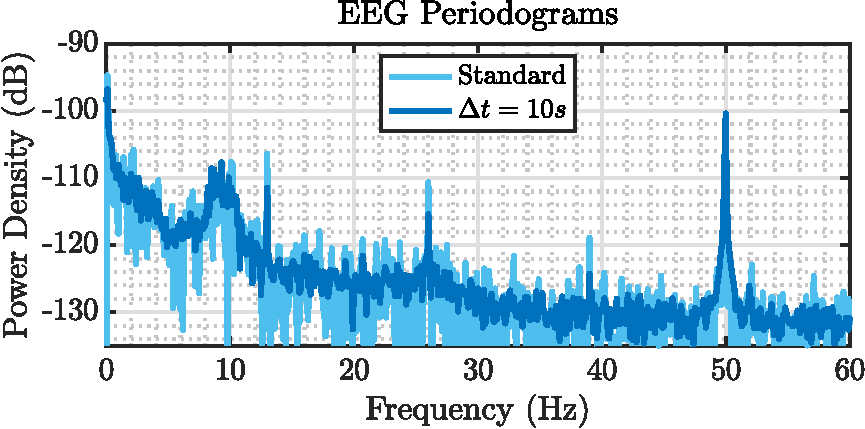
\includegraphics[height=1.5in]{report/spectrum-estimation/periodogram-based-methods-applied-to-real-world-data/assets/b/eeg-periodogram-averaged-bartlett-dt_10}
    \end{subfigure}
    ~ 
    \begin{subfigure}{0.49\textwidth}
        \centering
        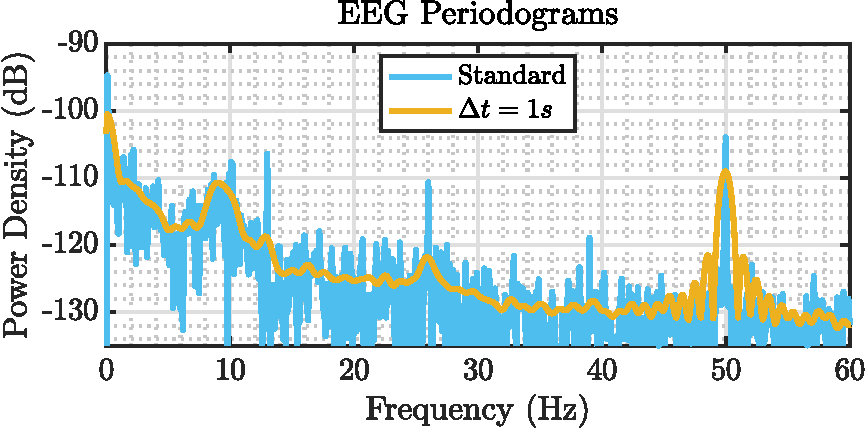
\includegraphics[height=1.5in]{report/spectrum-estimation/periodogram-based-methods-applied-to-real-world-data/assets/b/eeg-periodogram-averaged-bartlett-dt_1}
    \end{subfigure}
    \caption{EEG: Bartlett method periodogram averaging window $\Delta t$.}
    \label{fig:1_4_b_2}
\end{figure}

Figure \ref{fig:1_4_b_2} depicts the comparison between the Standard and Bartlett method periodograms for averagign window lengths $\Delta t = 10\ s$ and $\Delta t = 1\ s$.
For $\Delta t = 10\ s$, the periodogram has reduced variance compared to the standard periodogram, but inevitably reduced resolution. Nonetheless, the peaks of interest
(harmonics of SSEVP, power-line interference frequency and $8-10\ Hz$ band) are observable. On the other hand, for $\Delta t = 1\ s$ despite the even more reduced variance
(by a factor of 10) the resolution is insufficient to capture the $3^{rd}$ harmonic of SSEVP, but the rest of the peaks are visible.

Overall, the trade-off between variance and precision is illustrated, from the standard periodogram with best precision and maximum variance to the Bartlett method periodgram
with $\Delta t = 1\ s$ with worst precision and least variance.

%
\end{enumerate}